% This file was converted to LaTeX by Writer2LaTeX ver. 1.0.2
% see http://writer2latex.sourceforge.net for more info
\documentclass[twoside,letterpaper]{article}
\usepackage[latin1]{inputenc}
\usepackage[T1]{fontenc}
\usepackage[english]{babel}
\usepackage{amsmath}
\usepackage{amssymb,amsfonts,textcomp}
\usepackage{color}
\usepackage{array}
\newcolumntype{M}[1]{>{\centering\arraybackslash}m{#1}}
\usepackage{supertabular}
\usepackage{hhline}
\usepackage{hyperref}
\usepackage{float}
\hypersetup{pdftex, colorlinks=true, linkcolor=blue, citecolor=blue, filecolor=blue, urlcolor=blue, pdftitle=SOFTWARE REQUIREMENTS SPECIFICATION (SRS), pdfauthor=Shaylyn Adams}
\usepackage[pdftex]{graphicx}
% Outline numbering
\setcounter{secnumdepth}{5}
\renewcommand\thesection{\arabic{section}}
\renewcommand\thesubsection{\arabic{section}.\arabic{subsection}}
\renewcommand\thesubsubsection{\arabic{section}.\arabic{subsection}.\arabic{subsubsection}}
\renewcommand\theparagraph{\arabic{section}.\arabic{subsection}.\arabic{subsubsection}.\arabic{paragraph}}
\renewcommand\thesubparagraph{\arabic{section}.\arabic{subsection}.\arabic{subsubsection}.\arabic{paragraph}.\arabic{subparagraph}}
\makeatletter
\newcommand\arraybslash{\let\\\@arraycr}
\makeatother
% Page layout (geometry)
\setlength\voffset{-1in}
\setlength\hoffset{-1in}
\setlength\topmargin{0.5in}
\setlength\oddsidemargin{1in}
\setlength\evensidemargin{1in}
\setlength\textheight{8.278in}
\setlength\textwidth{6.5in}
\setlength\footskip{0.561in}
\setlength\headheight{0.5in}
\setlength\headsep{0.461in}
% Footnote rule
\setlength{\skip\footins}{0.0469in}
\renewcommand\footnoterule{\vspace*{-0.0071in}\setlength\leftskip{0pt}\setlength\rightskip{0pt plus 1fil}\noindent\textcolor{black}{\rule{0.25\columnwidth}{0.0071in}}\vspace*{0.0398in}}
% Pages styles
\makeatletter
\newcommand\ps@Standard{
  \renewcommand\@oddhead{\selectlanguage{english}\rmfamily\color{black} University of Massachusetts CICS \hfill \hfill Health-e}
  \renewcommand\@evenhead{\@oddhead}
  \renewcommand\@oddfoot{\foreignlanguage{english}{\textcolor{black}{SRS Page }}\foreignlanguage{english}{\textcolor{black}{\thepage{}}}}
  \renewcommand\@evenfoot{\@oddfoot}
  \renewcommand\thepage{\arabic{page}}
}
\newcommand\ps@Convertviii{
  \renewcommand\@oddhead{}
  \renewcommand\@evenhead{\@oddhead}
  \renewcommand\@oddfoot{}
  \renewcommand\@evenfoot{\@oddfoot}
  \renewcommand\thepage{\arabic{page}}
}
\newcommand\ps@Convertvii{
  \renewcommand\@oddhead{}
  \renewcommand\@evenhead{\@oddhead}
  \renewcommand\@oddfoot{}
  \renewcommand\@evenfoot{\@oddfoot}
  \renewcommand\thepage{\arabic{page}}
}
\newcommand\ps@Convertvi{
  \renewcommand\@oddhead{}
  \renewcommand\@evenhead{\@oddhead}
  \renewcommand\@oddfoot{}
  \renewcommand\@evenfoot{\@oddfoot}
  \renewcommand\thepage{\arabic{page}}
}
\newcommand\ps@Convertv{
  \renewcommand\@oddhead{}
  \renewcommand\@evenhead{\@oddhead}
  \renewcommand\@oddfoot{}
  \renewcommand\@evenfoot{\@oddfoot}
  \renewcommand\thepage{\arabic{page}}
}
\newcommand\ps@Convertiv{
  \renewcommand\@oddhead{}
  \renewcommand\@evenhead{\@oddhead}
  \renewcommand\@oddfoot{}
  \renewcommand\@evenfoot{\@oddfoot}
  \renewcommand\thepage{\arabic{page}}
}
\newcommand\ps@Convertii{
  \renewcommand\@oddhead{}
  \renewcommand\@evenhead{\@oddhead}
  \renewcommand\@oddfoot{}
  \renewcommand\@evenfoot{\@oddfoot}
  \renewcommand\thepage{\arabic{page}}
}
\newcommand\ps@FirstPage{
  \renewcommand\@oddhead{}
  \renewcommand\@evenhead{\@oddhead}
  \renewcommand\@oddfoot{}
  \renewcommand\@evenfoot{\@oddfoot}
  \renewcommand\thepage{\arabic{page}}
}
\makeatother
\pagestyle{Standard}
\setlength\tabcolsep{1mm}
\renewcommand\arraystretch{1.3}
% footnotes configuration
\makeatletter
\renewcommand\thefootnote{\arabic{footnote}}
\makeatother
\begin{document}
\clearpage\setcounter{page}{1}\pagestyle{Standard}
\thispagestyle{FirstPage}
\clearpage{\centering\selectlanguage{english}\bfseries\color{black}
SOFTWARE REQUIREMENTS SPECIFICATION (SRS) FOR 
\par}


\bigskip

{\centering\selectlanguage{english}\bfseries\color{black}
320 Green Team Project
\par}


\bigskip


\begin{figure}
\centering

\includegraphics[width=1.5in,height=1.5in]{Uma_seal.png}
\end{figure}

\bigskip


\bigskip

{\centering\selectlanguage{english}\bfseries\color{black}
Version 2.0
\par}

{\centering\selectlanguage{english}\bfseries\color{black}
November 9, 2015
\par}


\bigskip


\bigskip

{\centering\selectlanguage{english}\bfseries\color{black}
Prepared for:
\par}

{\centering\selectlanguage{english}\bfseries\color{black}
Sunderland/Leverett, MA Health Inspector
\par}


\bigskip


\bigskip

{\centering\selectlanguage{english}\bfseries\color{black}
Prepared by:
\par}

{\centering\selectlanguage{english}\bfseries\color{black}
Ather Akhtar, Andrew Chang, Peter Marathas, Andrew Marchetti, \par} 
{\centering\selectlanguage{english}\bfseries\color{black}
 Michael Markman, Eric Maryea, Neven Recchia,
\par}
{\centering\selectlanguage{english}\bfseries\color{black}
Shawn Sowersby, Alex Sullivan, and Josh Tranfaglia.\par}

{\centering\selectlanguage{english}\bfseries\color{black}
University of Massachusetts
\par}

{\centering\selectlanguage{english}\bfseries\color{black}
Amherst, MA \ 01003
\par}


\clearpage{\centering\selectlanguage{english}\bfseries\color{black}
\foreignlanguage{english}{\MakeUppercase{\ }}\foreignlanguage{english}{\MakeUppercase{320 
Green Team Project: Health-e}}
\par}

{\centering\selectlanguage{english}\bfseries\color{black}
TABLE OF CONTENTS
\par}


\bigskip

{\selectlanguage{english}\bfseries\color{black}
Section\ \hfill  Page}

\setcounter{tocdepth}{9}
\renewcommand\contentsname{}
\tableofcontents

\bigskip

\clearpage\clearpage\setcounter{page}{1}\pagestyle{Convertii}
\section[INTRODUCTION]{\selectlanguage{english}\rmfamily\bfseries\color{black}
INTRODUCTION}

\subsection[PURPOSE]{\selectlanguage{english}\rmfamily\bfseries\color{black}
PURPOSE}
{\selectlanguage{english}\rmfamily\color{black}
Replace the current physical method of archiving Board of Health data from restaurant inspections, well-water quality reports, and septic tank pumping reports with a new digital method. This document provides a high-level overview of the entire system before going into detail on the tablet application portion's form entry, browsing and search, and delayed upload functionality.
}


% \subsection[DOCUMENT CONVENTIONS]{\selectlanguage{english}\rmfamily\bfseries\color{black}
% DOCUMENT CONVENTIONS}
% {\selectlanguage{english}\rmfamily\color{black}
% Nothing needed here yet.}

\subsection[PRODUCT SCOPE]{\selectlanguage{english}\rmfamily\bfseries\color{black}
SCOPE}
{\selectlanguage{english}\rmfamily\color{black}
This project includes multiple sub-projects and systems. 
\\     \\
This new digital method requires a database to hold different types of inspection results and reports, including data on restaurants, well-water quality, and septic tanks. The database must be searchable and sortable by keywords or established parameters, thus improving accessibility and simplifying data analysis. Storing this data digitally will allow the customer to better analyze patterns and create a more accessible and interactive location for the data to reside. It will act as an intuitive tool to help the inspector use and access data in the future. To access this database, a user interface must be created to provide fast access and retrieval of information. This application focus on usability, with a sub-portion designed for portability. This application is meant to be used specifically in a municipality's Board of Health office environment. The application will include a convenient and easy method to search, sort, and analyze data from the restaurant inspections, well-water quality reports, and septic tank pumping reports. Septic tank and well-water quality data should also be viewable on a geographical map with the ability to show changes over time. This will illuminate differences and trends in the data that may help explain and predict them. The cataloging of restaurant health inspection data could be facilitated by a form on a portable application (i.e. mobile, tablet). This portable application should be designed to locally store the entered data and convert it to a form readable by the database so it can add the record to the rest of the database when connected.
\\     \\ 
Overall, creating and structuring a database for storing various health data, and providing easy-to-use tools for accessing it, will assist the customer in his inspections and simplify the retrieval of key information he may find interest in at a later date.
\subsubsection{Sub Projects}
\begin{itemize}
\item{Central Database}
\item{Form Entry Application for Tablet}
\item{Desktop Application}
\end{itemize}
\textit{Central Database:}
\newline 

A central database with constant access to data will ensure the integrity of the entire system. The three distinct data entities identified were: Well-water quality reports, septic system pumping reports, and restaurant inspections, which will all need to be differentiated by town. The attributes of the models will correspond to the required fields that the customer must enter during inspections. The data for the restaurant inspections shall contain all fields that can be found on the restaurant inspection form. The data for well reports must contain all of the relevant fields, such as water quality, measurements, address of water well, flow rate, name of the company that drilled the well, and the permit and lot number. Similarly, the data for the septic pumping report will hold information such as the address, lot number, size, capacity, condition of the tank, date of last inspection, and quality of gallons pumped in and out.  The type of data stored must be able to be changed in the event of new legislation.
\newline

The first of two sub-projects for creating this database are to create a basic database that provides basic queries, such as: creating, reading, editing, and deleting records safely and securely. The second sub-project is to create and design a method to federate the database so that other portions are able to access the database structure.
\\  \\
\textit{Form Entry Application for Tablet:}
\newline

This application will be focused on usability in order to make it as simple as possible to enter the data. The application will be able to store data locally on the device; and the ability to upload to the office-based application noted (e.g. desktop application or web-application). This app will replace the forms that the customer requires for every inspection by including fields for all relevant information. For security purposes, the app will have a log-in screen for user authentication. This application will be able to either send the document to a printer or email it on the spot, as well as be able to receive an e-signature. The application should allow the user to view relevant information based on data that is associated with the user's current task that has been submitted previously. For example, when the user is going to inspect a restaurant, they should be shown previous inspection results from that restaurant. 
\newline
\newline
The tablet application will have the following main sections that correspond with the functionality above: 
\begin{itemize}
\item{Data Entry with a user interface that allows for dynamic flow through the inspection process.}
\item{Geographic Information System (GIS) to locate well, septic, and restaurant locations.}
\item{Browsing and search of data in order to review previously entered reports for analysis purposes.}
\item{User authentication to verify identity of the user.}
\item{Form printing in order to leave any necessary paperwork after an inspection.}
\item{Delayed upload to save and move data without needing constant internet access}

\end{itemize}
\textit{Application (Usable, Connected to Database):}
\newline

An application will be created for viewing all past records stored in the database. The application should include three different sections for restaurant, wells, and septic systems.  The application will need to communicate with the central database containing all information of past records. The application will provide an interface for querying data, including searching by location or violation. The application will contain user authentication that, once validated as an administrator, will allow for the submission of new records. Without log-in credentials, the information will be visible, but immutable. The application will use the accepted regulation forms as a base to record data from new restaurant inspection, water, or septic system reports and then send this new data to the relevant database. Additional functionality of this application includes:
\newline 
\begin{itemize}
\item{Reporting and search that includes many enter-able parameters to view and categorize reports}
\item{User authentication so that inspectors can add report data and constituents may view public records.}
\item{Data mapping to view data in relation to maps of corresponding towns.}
\item{Printing of reports or search results for when physical copies are desired.}
\end{itemize}
}

\subsection[INTENDED AUDIENCE]{\selectlanguage{english}\rmfamily\bfseries\color{black}
INTENDED AUDIENCE}
{\selectlanguage{english}\rmfamily\color{black}
    This system is intended for health inspectors who want to use a digital alternative to record and store information as opposed to paper storage. Specifically, the system is being made for the health inspector of the towns of Leverett and Sunderland, Massachusetts.}

\subsection[DEFINITIONS, ACRONYMS, AND
ABBREVIATIONS]{\selectlanguage{english}\rmfamily\bfseries\color{black}
DEFINITIONS, ACRONYMS, AND ABBREVIATIONS}
{\selectlanguage{english}\rmfamily\color{black}
The product's name is Health.e standing for Health Electronics, as it is designed to digitize information on health inspections, well water reports and septic tank pumpings.}
\newline
\begin{flushleft}
\tablehead{}
\begin{supertabular}{|m{1.3587599in}|m{5.00806in}|}
\hline
\centering \selectlanguage{english}\bfseries\color{black} Term or
Acronym &
\centering\arraybslash \selectlanguage{english}\bfseries\color{black}
Definition\\\hline
\selectlanguage{english}\color{black} DFD &
\selectlanguage{english}\color{black} Data Flow Diagram\\\hline
\selectlanguage{english}\color{black} SRS &
\selectlanguage{english}\color{black} Software Requirements
Specification\\\hline
\selectlanguage{english}\color{black} GIS &
\selectlanguage{english}\color{black} Geographic Information System\\\hline
\end{supertabular}
\end{flushleft}

% \subsection[REFERENCESS]{\selectlanguage{english}\rmfamily\bfseries\color{black}
% REFERENCES}
% {\selectlanguage{english}\itshape\color{black}
% WRITE HERE}


\clearpage\section[OVERALL
DESCRIPTION]{\selectlanguage{english}\rmfamily\bfseries\color{black}
OVERALL DESCRIPTION}

\subsection[PRODUCT
PERSPECTIVE]{\selectlanguage{english}\rmfamily\bfseries\color{black}
PRODUCT PERSPECTIVE}
This product will be replacing the primary user's current pen and paper system for documenting inspections. Rather than filling out paper forms on site and handing the inspectee a carbon copy of the form, the tablet app will allow the inspector to collect the same data and print a standard form from a portable printer on site for the inspectee to review. Also, rather than storing paper files in a filing cabinet that may never be looked at again, the health inspector may, with our product, review previous forms with ease by searching for them with our comprehensive browsing and search functionality. This way, records may be found in a matter of seconds. Another aspect of this product will be the delayed upload in which forms that have been filled out on the tablet and stored locally will be synced with the central database so that they may be integrated with the main application. This eliminates the need for the health inspector to ''file'' each form after completing it.
\newline
The form entry, browsing and search, and delayed upload functionalities are all subprojects for the entire tablet app, which is, in and of itself, a subproject of the main project. Our contribution to the main project is depicted below:

\begin{figure}[H]
\centering
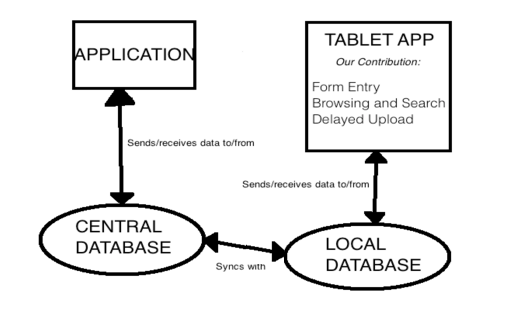
\includegraphics[width=4in,height=3in]{Diagram1.png}
\end{figure}


\subsection[PRODUCT
FUNCTIONS]{\selectlanguage{english}\rmfamily\bfseries\color{black}
PRODUCT FUNCTIONS}
\subsubsection{Data Entry (Forms)}
\begin{enumerate}
\item{The user chooses one of the following data forms to fill in: restaurant, septic tank, or water well.}
\item{The tablet then displays the chosen form to the user with blank, fillable forms.}
\end{enumerate}
\subsubsection{Browsing \& Search}
\begin{enumerate}
\item{The user types in a location of the desired restaurant, septic tank, or water well.}
\item{The tablet displays records from its database relevant to the search requirements.}
\end{enumerate}
\subsubsection{Delayed Upload}
\begin{enumerate}
\item{The tablet synchronizes with the external database and uploads either specific or all records from the tablet to the external database once a connection has been established.}
\end{enumerate}

\subsection[USER
CHARACTERISTICS]{\selectlanguage{english}\rmfamily\bfseries\color{black}
USER CHARACTERISTICS}
{\selectlanguage{english}\rmfamily\color{black}
The form entry, browsing and search, and delayed upload parts of the tablet will primarily be used by health inspectors. They will have full access to all functional aspects listed in section 2.2. Unregistered guests will have limited, read-only access to the main application of the project while only the registered health inspectors may access the tablet application.}

\subsection[OPERATING ENVIRONMENT]{\selectlanguage{english}\rmfamily\bfseries\color{black}
OPERATING ENVIROMENT}
{\selectlanguage{english}\rmfamily\color{black}
The form entry, browsing and search, and delayed upload aspects of this project will all exist on the same platform: a tablet. The tablet should have a small amount of memory allocated to the app so that data records may be stored locally until uploaded to the central database.}



\subsection[CONSTRAINTS]{\selectlanguage{english}\rmfamily\bfseries\color{black}
CONSTRAINTS}
\subsubsection{Data Entry (Forms)}
{\selectlanguage{english}\color{black}
The form entry itself is primarily based on inspection forms created by the state and used by the town. There must be an entry field for each piece of data corresponding to the required sections of the current inspection forms. Also, there will be a finite number of form entries the user can generate on the tablet since the tablet will have a limited amount of memory space. With recent tablet device improvements, the chances of filling up the memory on the tablet is low. With a good design of the entire project, modern day memory capacities will suffice to hold the data required.}

\subsubsection{Browsing \& Search}
{\selectlanguage{english}\color{black}
Browsing and searching features are constrained by the design of the database itself. With a good design and structure, these features will be user-intuitive and minimal effort will be needed by the user to use these features. Browsing and searching the form entries is constrained by the number of form entries in the database on the tablet.}

\subsubsection{Delayed Upload}
{\selectlanguage{english}\color{black}
The delayed upload is constrained by the health inspector's access to WiFi or some form of manual docking technology. Either method may be used in order for the local memory on the tablet to sync with the central database, but one must exist.}

\subsection[USER DOCUMENTATION]{\selectlanguage{english}\rmfamily\bfseries\color{black}
USER DOCUMENTATION}
{\selectlanguage{english}\rmfamily\color{black}
There will be a GitHub Wiki that will help guide the user through all of the basic functionality of the tablet app, and in general, the application as a whole. The Wiki will be user friendly, easily comprehensible, and will touch on all of the important features of the app that the primary user should be familiar with.}

\subsection[ASSUMPTIONS \& DEPENDENCIES]{\selectlanguage{english}\rmfamily\bfseries\color{black}
ASSUMPTIONS \& DEPENDENCIES}
\subsubsection{Data Entry (Forms)}
Our implementation of the form entry on the tablet app depends on how the central database is constructed. Each field that the database contains for each type of form must be represented in the UI of the tablet app so that the health inspector may enter all of the fields correctly. The assumption here being that any changes made to the physical forms will be updated accordingly in the database, and thus updated in the digital forms as well. 
\subsubsection{Browsing \& Search}
Our implementation of browsing and search on the tablet app relies on an internal database that holds previous records. We assume that the internal database is synced with the main database, so that the files being searched for can be found within the tablet. There is a possibility that files that have been removed from the tablet may be searched for, but such a case will be handled by a file not found message. 
\subsubsection{Delayed Upload}
We are assuming that the health inspector will have WiFi access in order for the tablet app to upload data from its local database to the central database via a syncing process. In the case that this assumption is incorrect and the user does not have WiFi access, a manual docking process will have to occur between the tablet and the health inspector's computer on which the main application exists. This assumes that the health inspector has the proper cable to connect the tablet to said computer, but this is a reasonable assumption since such a cable typically is included with the purchase of a tablet since its serves the dual purpose of a charger. The delayed upload also depends on the construction of the database and its fields as well as the application itself since it must sync with said application.

\clearpage\section[EXTERNAL INTERFACE
REQUIREMENTS]{\selectlanguage{english}\rmfamily\bfseries\color{black}
EXTERNAL INTERFACE
REQUIREMENTS}

\subsection[USER INTERFACES]{\selectlanguage{english}\rmfamily\bfseries\color{black}
USER INTERFACES}
{\selectlanguage{english}\rmfamily\color{black}
The user interface for the system will be an app based application on a tablet. The user will enter log-in parameters as user authentication. The user will then be able to select which records to access. The user will be able to enter record data in the app on the replicated forms for the inspection. The user will also be able to send the document to a printer or email it. The app will also have the ability for the user to browse and search for information on the app. The user will be able to select for a delayed upload as well.}

\subsection[HARDWARE INTERFACES]{\selectlanguage{english}\rmfamily\bfseries\color{black}
HARDWARE INTERFACES}
{\selectlanguage{english}\rmfamily\color{black}
  The hardware interfaces of the system will be run on an android device. An internet connection will allow the software interfaces to connect to the internet and sync with records in the database. The tablet will also contain a local database allowing for complete offline access of previous record entry.  }

\subsection[SOFTWARE INTERFACES]{\selectlanguage{english}\rmfamily\bfseries\color{black}
SOFTWARE INTERFACES}
{\selectlanguage{english}\rmfamily\color{black}
\subsubsection{Operating System} 
The software is being designed to run on Ionic. Ionic is a tool that is written in html, css, and javascript allowing for a web-app, ios-app- and android-app to be developed at once.
\subsubsection{Web Server}
The software will be able to sync with a database as well as contain its own personal database. This will allow for consistent access to previously recorded data. The web server and local database will be synchronized with a consistent data-model. 
\subsubsection{Database}
The software will use a federated database to store all the data. This federated database will allow for the decentralization of the two towns, Sunderland and Leverett but also provide access to all records through a common API. }

\subsection[COMMUNICATION INTERFACES]{\selectlanguage{english}\rmfamily\bfseries\color{black}
COMMUNICATION INTERFACES}
{\selectlanguage{english}\rmfamily\color{black}

\subsubsection{Form Interface}
The application will provide electronic entries that the user needs. These entries will be modeled after the forms provided by the customer and provide the ability for the customer to submit an entry in any order required.

\subsubsection{Web Communication}
The application will be able to wirelessly sync with the database. This feature will not be the only syncing mechanism but will provide an alternative to how data is uploaded. All syncing will interact through the web application which will allow the database to only interact with a single entity (the web application) thus preventing any write conflicts between the tablet and web application.

\subsubsection{USB Communication}
The application will be able to sync through a usb cable with the database. This hard wire connection will provide full autonomy for the customer to upload specific forms to the web application. The USB connection will also be able to read from the computer in order to update attributes on the tablets local database.}

\clearpage\section[NON-FUNCTIONAL REQUIREMENTS]{\selectlanguage{english}\rmfamily\bfseries\color{black}
NON-FUNCTIONAL REQUIREMENTS}
{\selectlanguage{english}\rmfamily\color{black}

\subsection{SOFTWARE QUALITY ATTRIBUTES}
The most important aspect of the final product is that it must be extremely user-friendly. Operating the software should be a simple and intuitive process. A new user should be able to learn how to operate the software very quickly. Learning how to use this software is not the job, but the tool to accomplishing the job easily and effectively.

\subsection{PERFORMANCE REQUIREMENTS}
The software must operate efficiently enough such that it does not cause delay during an inspection. Operation of the software should be quick and responsive in order to satisfy the user's needs.

\subsection{SAFETY REQUIREMENTS}
We must operate under the assumption that the application may be offline for some amount of time. During this time, all data saved on the tablet must remain organized and secure. During any instance of Delayed Upload, data must remain intact and the connection must be secure such that no corruptions or issues arise.

\subsection{SECURITY REQUIREMENTS}
It is vital that data entry is only accessible to authorized users. User authentication should ensure that only administrators can enter information into the database. While the data on the tablet will eventually become open to the public, this part of the application should be restricted to inspectors.}

\clearpage\section[FUNCTIONAL REQUIREMENTS]{\selectlanguage{english}\rmfamily\bfseries\color{black}
FUNCTIONAL REQUIREMENTS}
\subsection[DATA ENTRY (FORMS)]{\selectlanguage{english}\rmfamily\bfseries\color{black}
DATA ENTRY (FORMS)}

\subsubsection{\textit{Use Case 1}}

\textit{Title: }{\selectlanguage{english}\bfseries\color{black} Fill out septic tank pumping data form}

{\selectlanguage{english}\color{black} \textit{Primary Actor:} User}

{\selectlanguage{english}\color{black} \textit{Secondary Actor:} System}

{\selectlanguage{english}\color{black} \textit{Trigger:} User selects septic pumping data form.}

{\selectlanguage{english}\color{black} \textit{Precondition:} User  successfully logged in and accessed the form entry user interface for the septic tank.}

{\selectlanguage{english}\color{black} \textit{Postcondition:}  Data is stored to be submitted to a central database}
\newline

{\selectlanguage{english}\color{black} \textit{Main Scenario:}}
\begin{enumerate}
\item System presents modifiable septic tank information form.

\item User fills out fields on the form.

\item User submits the form on tablet.

\item System determines that each required and non-required field entered is valid.

\item System creates an accessible local copy.

\item System displays a response when successfully entering form.

\item User safely closes out of process (data is preserved).
\end{enumerate}

{\selectlanguage{english}\color{black} \textit{Exception Scenario:}}
\begin{enumerate}
\item User forgets to enter information in 'required field'.
\begin{enumerate}
\item System notifies user of empty fields and goes back to step 2.
\end{enumerate}

\item User enters an invalid form entry.
\begin{enumerate}
\item System displays invalid form entry and goes back to step 2.
\end{enumerate}

\item System shuts down during data submission.
\begin{enumerate}
\item System can show user whether or not data was submitted successfully. 
\end{enumerate}

\item User cancels form entry.
\begin{enumerate}
\item User selects cancel option.
\item System confirms with user that they selected cancel.
\item System displays main application screen.

\end{enumerate}
\end{enumerate}


\subsubsection{\textit{Use Case 2}} 

\textit{Title: }{\selectlanguage{english}\bfseries\color{black} Fill out well water data form}

{\selectlanguage{english}\color{black} \textit{Primary Actor:} User}

{\selectlanguage{english}\color{black} \textit{Secondary Actor:} System}

{\selectlanguage{english}\color{black} \textit{Trigger:} User selects well water data form.}

{\selectlanguage{english}\color{black} \textit{Precondition:} Successfully logged in and accessed the form entry user interface for water wells.}

{\selectlanguage{english}\color{black} \textit{Postcondition:}  Data is stored to be submitted to a central database}
\newline

{\selectlanguage{english}\color{black} \textit{Main Scenario:}}
\begin{enumerate}
\item System presents modifiable well water information form.

\item User fills out fields on the form.

\item User submits the form on tablet.

\item System determines that each required and non-required field entered is valid.

\item System allocates memory and creates an accessible local copy.

\item System displays a response when successfully entering form.

\item User safely closes out of process (data is preserved).
\end{enumerate}

{\selectlanguage{english}\color{black} \textit{Exception Scenarios:}}
\begin{enumerate}
\item User forgets to enter information in 'required field'.
\begin{enumerate}
\item System notifies user of empty fields and does not submit.
\item User presented with partially filled out form and goes back to step 2.
\end{enumerate}

\item User enters an invalid form entry.
\begin{enumerate}
\item System displays invalid form entry and does not submit.
\item User presented with partially filled out form and goes back to step 2.
\end{enumerate}

\item System shuts down during data submission.
\begin{enumerate}
\item System shows user whether or not data was submitted successfully.
\end{enumerate}

\item User cancels form entry.
\begin{enumerate}
\item User selects cancel option.
\item System confirms with user that they selected cancel.
\item System displays main application screen.
\end{enumerate}
\end{enumerate}

\subsubsection{\textit{Use Case 3}}

\textit{Title: }{\selectlanguage{english}\bfseries\color{black} Fill out restaurant inspection form}

{\selectlanguage{english}\color{black} \textit{Primary Actor:} User}

{\selectlanguage{english}\color{black} \textit{Secondary Actor:} System}

{\selectlanguage{english}\color{black} \textit{Trigger:} User selects restaurant inspection form to fill out.}

{\selectlanguage{english}\color{black} \textit{Precondition:} User has passed login authentication, and has chosen to submit data for a restaurant inspection.}

{\selectlanguage{english}\color{black} \textit{Postcondition:}  Data is stored to be submitted to a central database}
\newline

{\selectlanguage{english}\color{black} \textit{Main Scenario:}}
\begin{enumerate}
\item The page for restaurant inspection form is shown.
\item User chooses restaurant.
\item User fills out fields in form to record data from inspection.
\item User clicks save button.
\item Data is stored locally.
\end{enumerate}

{\selectlanguage{english}\color{black} \textit{Exception Scenario:}}
\begin{enumerate}
\item User forgets to enter information in 'required field'.
\begin{enumerate}
\item System notifies user of empty fields and does not submit.
\item User presented with partially filled out form and go back to step 3.
\end{enumerate}

\item User enters an invalid form entry.
\begin{enumerate}
\item System displays invalid form entry and does not submit.
\item User presented with partially filled out form and go back to step 3.
\end{enumerate}

\item System shuts down during data submission.
\begin{enumerate}
\item System shows user whether or not data was submitted successfully. 
\end{enumerate}

\item User cancels form entry.
\begin{enumerate}
\item User selects cancel option.
\item System confirms with user that they selected cancel.
\item System displays main application screen.
\end{enumerate}
\end{enumerate}


\subsubsection{\textit{Use Case 4}} 

\textit{Title: }{\selectlanguage{english}\bfseries\color{black} Enter new restaurant inspection form}

{\selectlanguage{english}\color{black} \textit{Primary Actor:} User}

{\selectlanguage{english}\color{black} \textit{Secondary Actor:} System}

{\selectlanguage{english}\color{black} \textit{Trigger:} User selects restaurant inspection form.}

{\selectlanguage{english}\color{black} \textit{Precondition:} Successfully logged in and accessed the form entry user interface for restaurant inspection.}

{\selectlanguage{english}\color{black} \textit{Postcondition:}  Filling out restaurant form now has option to select this new restaurant}
\newline

{\selectlanguage{english}\color{black} \textit{Main Scenario:}}
\begin{enumerate}
\item The page for restaurant inspection form is shown.

\item User selects "add new restaurant" option, which resides next to "restaurant name" field.

\item System redirects user to "new restaurant" form.

\item User enters restaurant information; includes name, address, owner, etc.

\item User hits submit button after all fields have been entered.

\item System redirects User back to restaurant inspection page.

\item User has option to select the new restaurant from list of restaurants under "restaurant name".

\end{enumerate}

{\selectlanguage{english}\color{black} \textit{Exception Scenarios:}}
\begin{enumerate}
\item User forgets to enter information in 'required field'.
\begin{enumerate}
\item System notifies user of empty fields and does not submit.
\item User presented with partially filled out form and goes back to step 3.
\end{enumerate}

\item User enters an invalid form entry.
\begin{enumerate}
\item System displays invalid form entry and does not submit.
\item User presented with partially filled out form and goes back to step 3.
\end{enumerate}

\item System shuts down during data submission.
\begin{enumerate}
\item System shows user whether or not data was submitted successfully.
\end{enumerate}

\item User cancels form entry.
\begin{enumerate}
\item User selects cancel option.
\item System confirms with user that they selected cancel.
\item System redirects User back to restaurant inspection form page.
\end{enumerate}
\end{enumerate}

\subsection[BROWSING \& SEARCH]{\selectlanguage{english}\rmfamily\bfseries\color{black}
BROWSING \& SEARCH}

\subsubsection{\textit{Use Case 1}}

\textit{Title: }{\selectlanguage{english}\bfseries\color{black} Search for prior report}

{\selectlanguage{english}\color{black} \textit{Primary Actor:} User}

{\selectlanguage{english}\color{black} \textit{Secondary Actor:} System}

{\selectlanguage{english}\color{black} \textit{Trigger:} User wants to search for a list of inspection reports matching an entered keyword.}

{\selectlanguage{english}\color{black} \textit{Preconditions:} User has logged in and is on the initial lookup report screen which contains a list of all reports.}

{\selectlanguage{english}\color{black} \textit{Postcondition:} System displays list of prior reports matching search term.}
\newline

{\selectlanguage{english}\color{black} \textit{Main Scenario:}}
\begin{enumerate}
\item User enters a keyword to search.
\item System queries external database with location and retrieves records that contain the keyword.
\item System displays a list of retrieved records and their dates, sorted by date.
\end{enumerate}

{\selectlanguage{english}\color{black} \textit{Exception Scenarios:}}
\begin{enumerate}
\item System cannot connect to database.
\begin{enumerate}
\item Screen displays connection error message and asks user to try again later.
\item User selects 'Ok' button and system returns to the lookup report screen.
\end{enumerate}

\item None of the records match the search keyword.
\begin{enumerate}
\item Display message, ''No reports match the specified keyword''.
\item User clicks 'Ok' and returns to the initial lookup report screen.
\end{enumerate}
\end{enumerate}

\subsubsection{\textit{Use Case 2}}

\textit{Title: }{\selectlanguage{english}\bfseries\color{black}Narrow down list of inspection reports}

{\selectlanguage{english}\color{black} \textit{Primary Actor:} User}

{\selectlanguage{english}\color{black} \textit{Secondary Actor:} System}

{\selectlanguage{english}\color{black} \textit{Trigger:} User wants to select criteria to narrow down a list of all inspection reports.}

{\selectlanguage{english}\color{black} \textit{Preconditions:} User has logged in and is on the initial lookup report screen which contains a list of all inspection reports.}

{\selectlanguage{english}\color{black} \textit{Postcondition:} System displays list of prior reports matching the selected criteria.}
\newline
{\selectlanguage{english}\color{black} \textit{Main Scenario:}}\
\begin{enumerate}
\item User selects criteria to narrow down all the inspection reports.
\item System queries external database with location and retrieves records that match the criteria.
\item System displays a list of retrieved records and their dates, sorted by date.
\end{enumerate}
{\selectlanguage{english}\color{black} \textit{Exception Scenarios:}}
\begin{enumerate}
\item System cannot connect to database.
\begin{enumerate}
\item Screen displays connection error message and asks user to try again later.
\item User selects 'Ok' button and system returns to the lookup report screen.
\end{enumerate}

\item None of the records match the search keyword.
\begin{enumerate}
\item Display message, ''No reports matching that criteria''.
\item User clicks 'Ok' and returns to the initial lookup report screen.
\end{enumerate}
\end{enumerate}

\subsubsection{\textit{Use Case 3}}

\textit{Title: }{\selectlanguage{english}\bfseries\color{black}View an inspection report}

{\selectlanguage{english}\color{black} \textit{Primary Actor:} User}

{\selectlanguage{english}\color{black} \textit{Secondary Actor:} System}

{\selectlanguage{english}\color{black} \textit{Trigger:} User wants to view a specific inspection report.}

{\selectlanguage{english}\color{black} \textit{Preconditions:} User has logged in and is on the lookup report screen which contains a list inspection reports.}

{\selectlanguage{english}\color{black} \textit{Postcondition:} System displays the selected inspection report.}
\newline
{\selectlanguage{english}\color{black} \textit{Main Scenario:}}\
\begin{enumerate}
\item User selects an inspection report.
\item System displays all data contained in the selected inspection report.
\end{enumerate}
{\selectlanguage{english}\color{black} \textit{Exception Scenario:}}

\begin{description}
\item System cannot connect to database.
\begin{enumerate}
\item Screen displays connection error message and asks user to try again later.
\item User selects 'Ok' button and system returns to the lookup report screen.
\end{enumerate}
\end{description}

\subsection[DELAYED UPLOAD]
{\selectlanguage{english}\rmfamily\bfseries\color{black}
DELAYED UPLOAD}
\subsubsection{\textit{Use Case 1}}

\textit{Title: }{\selectlanguage{english}\bfseries\color{black}User attempts to upload a record.}

{\selectlanguage{english}\color{black} \textit{Primary Actor:} System}

{\selectlanguage{english}\color{black} \textit{Secondary Actor:} User}

{\selectlanguage{english}\color{black} \textit{Trigger:} User selects record/inspection to upload.}

{\selectlanguage{english}\color{black} \textit{Precondition:}User has completed and saved some type of form data, and is associated with some online database. User is on the start page and has signed in successfully. Alternatively, User opts to send form data immediately after saving to device and begins at step 2.}

{\selectlanguage{english}\color{black} \textit{Postcondition:}Form data has not already been submitted to the database and is added successfully. If conditions are not correct for proper form data upload, data is not uploaded.}
\newline

{\selectlanguage{english}\color{black} \textit{Main Scenario:}}
\begin{enumerate}
\item User navigates the form data on the application to find the data they desire to upload.
\item User indicates that they want to upload the form data.
\item System verifies that the form data is acceptable for submission to online database.
\item System verifies that internet connection is available.
\item System verifies that connection to associated database is available.
\item System verifies that given form data has not already been submitted to the database.
\item System asks the user for confirmation to send the form data.
\item User gives confirmation of intent to send the form data
\item System adds the new form data to the database using the internet connection available.
\item System notifies the user of successful upload of the data.
\end{enumerate}

{\selectlanguage{english}\color{black} \textit{Exception Scenario:}}

\begin{enumerate}
\item Form data is not acceptable for upload.
\begin{enumerate}
\item System notifies the user that the form data is not acceptable for upload. System 
specifies which fields in the form data are unacceptable and asks that they be fixed before submission.
\item User is returned to the form's viewing page.
\end{enumerate}

\item No internet connection is available.
\begin{enumerate}
\item System notifies the user that internet connection is not available and to try again once they are within access range.
\item User is returned to the form's viewing page.
\end{enumerate}

\item Only internet connections that are available are not Wi-Fi connections.
\begin{enumerate}
\item System asks the user to verify that they would like to send the connection on the mobile network.
\item If user accepts, use case proceeds as normal at step 4.
\item If user refuses, system notifies the user to try uploading again once they are within access range.
\item User is returned to the form's viewing page.
\end{enumerate}

\item System is unable to connect with the database.
\begin{enumerate}
\item System notifies the user that it is impossible to connect to the database and to verify that the database is online.
\item User is returned to the form's viewing page.
\end{enumerate}

\item Form data has already been submitted to the database.
\begin{enumerate}
\item System notifies the user that the form has already been uploaded before.
\item User is returned to the form's viewing page.
\end{enumerate}

\item User declines the confirmation to send the data.
\begin{enumerate}
\item Form data is not sent. User is returned to the form's viewing page.
\end{enumerate}

\item No internet connection is available.
\begin{enumerate}
\item System notifies the user that internet connection is not available and to try again once they are within access range.
\item User is returned to the form's viewing page.
\end{enumerate}
\end{enumerate}

\subsubsection{\textit{Use Case 2}}

\textit{Title: }{\selectlanguage{english}\bfseries\color{black}Batch upload all forms that are not already uploaded.}

{\selectlanguage{english}\color{black} \textit{Primary Actor:} System}

{\selectlanguage{english}\color{black} \textit{Secondary Actor:} User, Databse}

{\selectlanguage{english}\color{black} \textit{Trigger:} User selects record/inspection to upload.}

{\selectlanguage{english}\color{black} \textit{Precondition:}  User has completed and saved some type of form data, and the device is associated with some online database. User is on the start page and has signed in successfully. Alternatively, setting for automatic upload is on and System engages automatically, starting at step 2.}

{\selectlanguage{english}\color{black} \textit{Postcondition:} Form data that has not already been submitted to the database and is acceptable for upload is added successfully. If conditions are not correct for proper form data upload, data is not uploaded.}

{\selectlanguage{english}\color{black} \textit{Main Scenario:}}
\begin{enumerate}
\item User indicates that they would like to perform a batch upload of form data.
\item System verifies that internet connection is available.
\item System verifies that connection to associated database is available.
\item System cross-references form data on the device and on the database to find which data is on the device and not in the database.
\item System displays a list of the eligible form data on the device and requests the user confirms the data.
\item User selects the data they wish to upload to the database and confirms to send those forms.
\item System checks each data that is desired to be uploaded is acceptable to be added to the database.
\item System sends acceptable form data to the database to be added.
\item System notifies the user of which form data was successfully sent to the database.
\end{enumerate}

{\selectlanguage{english}\color{black} \textit{Exception Scenario:}}
\begin{enumerate}
\item No internet connection is available.
\begin{enumerate}
\item System notifies the user that internet connection is not available and to try again once they are within access range.
\item User is returned to the main viewing page.
\end{enumerate}

\item Only internet connections that are available are not Wi-Fi connections.
\begin{enumerate}
\item System asks the user to verify that they would like to send the connection on the mobile network.
\item If user accepts, use case proceeds as normal at step 3.
\item If user refuses, system notifies the user to try uploading again once they are within access range.
\item User is returned to the main viewing page.
\end{enumerate}

\item System is unable to connect with the database.
\begin{enumerate}
\item System notifies the user that it is impossible to connect to the database and to verify that the database is online.
\item User is returned to the main viewing page.
\end{enumerate}

\item All form data on the device is also on the database.
\begin{enumerate}
\item System notifies the user that there is no data to be upload to the database.
\item User is returned to the main viewing page.
\end{enumerate}

\item User declines to upload data.
\begin{enumerate}
\item User is returned to the main page.
\end{enumerate}

\item Some form data is not acceptable to be uploaded to the database.
\begin{enumerate}
\item Any data that is not acceptable is removed from the list of data to be uploaded. After batch upload is finished, a notification is sent with a list of any data unacceptable to be uploaded.
\item System displays main application screen.
\end{enumerate}

\item No internet connection is available.
\begin{enumerate}
\item System notifies the user that internet connection is not available and to try again once they are within access range.
\item User is returned to the main viewing page.
\end{enumerate}

\item System is unable to connect with the database.
\begin{enumerate}
\item System notifies the user that it is impossible to connect to the database and to verify that the database is online.
\item User is returned to the main viewing page.
\end{enumerate}
\end{enumerate}

\clearpage\section[DATA MODELING]{\selectlanguage{english}\rmfamily\bfseries\color{black}
DATA MODELING}
\subsection{DATA DESCRIPTION}
{\selectlanguage{english}\rmfamily\color{black}
Data from three objects and their respective fields are collected from the user and stored in the database.  Objects are searched using fields.  Search results in data in the form of objects being output from the database.}

\begin{figure}[H]
\centering
\renewcommand{\figurename}{DFD}
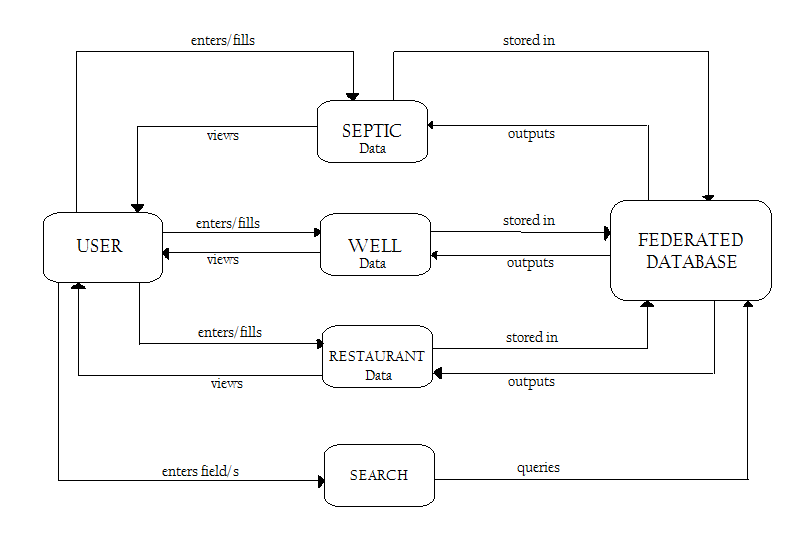
\includegraphics[width=4in,height=3in]{Diagram2.png}
\end{figure}

\subsection{DATA OBJECTS}
Three different data objects and their fields are stored in the database; septic pumping form, water well inspection form, and restaurant inspection forms.  Users use search object and its field to query the database.
\begin{itemize}
\item{Septic tank:}  Septic tank objects holds fields and data from septic tank pumping forms.  These objects are stored in the database and can retrieved using search options.

\item{Water Well:} Water well object holds fields and data from water well inspection forms.  These objects are stored in the database and can retrieved using search options.

\item{Restaurant:} Restaurant object holds fields and data from restaurant inspection forms.  These objects are stored in the database and can retrieved using search options.

\item{Search:} Search object holds the fields entered by the user during search process.  Database matches the fields from the search object to the corresponding stored objects and fields to output the results.
\end{itemize}

\clearpage\section[TEST PLAN]{\selectlanguage{english}\rmfamily\bfseries\color{black}
TEST PLAN}

\subsection{OBJECTIVES}
{\selectlanguage{english}\rmfamily\color{black}
 The objective of the test plan is to ensure a high level of confidence in the correctness and usefulness of the project deliverables.}

\subsection{TESTING STRATEGY}
{\selectlanguage{english}\rmfamily\color{black}
        The strategy for testing the softwares data entry, browsing and search, and delayed update features is a combination of automation testing and manual testing. Functional requirements of the listed features are to be tested by using automation testing. Manual testing will only be used for features that may not be testable by automation. Certain components of these features may involve more intensive interaction between the tablet and the user and these components will need validation by testers and developers.}
        
\subsection{SCOPE}
{\selectlanguage{english}\rmfamily\color{black}
       Testing for this section will be conducted throughout the development life cycle of the product.
}

\subsection{FEATURES TO BE TESTED}
{\selectlanguage{english}\rmfamily\color{black}
Test cases will cover all the features of the software covered in the SRS.  It will include the exception cases in the use cases so as to ensure that the product behaves in the anticipated manner.
}

\begin{center}
\begin{tabular}{ | M{1.5cm} | M{1.75cm}| M{13cm} |} 
\hline
\textbf{TEST ID} & \textbf{SRS \ Document \ Reference} & \textbf{Features To Be Tested (Test Description)}\\ 
\hline
001 & 5.1.1 & Validate the data entry form feature for septic tanks. Test cases will ensure that the user is able to input and upload the form in the expected manner.  Test cases will also test for exceptions: 1) User misses a required  entry, 2) User inputs invalid entry 3) System shutdown during data upload.\\ 
\hline
002 & 5.1.2 & Validate the data entry form feature for water well. Test cases will ensure that the user is able to input and upload the form in the expected manner.  Test cases will also test for exceptions: 1) User misses a required  entry, 2) User inputs invalid entry 3) System shutdown during data upload. \\ 
\hline
003 & 5.1.3 & Validate the data entry form feature for restaurant inspections. Test cases will ensure that the user is able to input and upload the form in the expected manner.  Test cases will also test for exceptions: 1) User misses a required  entry, 2) User inputs invalid entry 3) System shutdown during data upload. \\ 
\hline
004 & 5.2 & Validate the browsing and search functions. Test cases will include scenarios for software not able to connect to database and search query yielding no results.\\ 
\hline
005 & 5.3.1 & Validate the delayed upload feature for specific form selected by user.  Test cases will include tests for exceptional scenarios covered in SRS to ensure that the software behaves in an expected manner.\\ 
\hline
006 & 5.3.2 & Validate the batch delayed upload feature.  Test cases will include tests for exceptional scenarios covered in SRS to ensure that the software behaves in an expected manner.\\ 
\hline
\end{tabular}
\end{center}

\subsection{APPROACH}

\begin{center}
\begin{tabular}{ | M{4cm} | M{12cm}| } 
\hline
\textbf{Component Testing} & Components will be tested by test cases to ensure they are working during the software development cycle.\\ 
\hline
\textbf{Integration Testing} & A detailed set of test cases will be created and then executed.  These test cases will cover all the requirements detailed in the SRS.\\ 
\hline
\textbf{Interface Testing} & To ensure that all aspects of the display are rendered correctly, the external interfaces regarding data entry forms and browsing and searching will be tested manually by using the user interface to perform all product tasks.\\ 
\hline
\textbf{Security Testing} & Security of the software will be tested by making attempts to access the data without proper authentication.\\ 
\hline
\textbf{Performance Testing} & Test users will interact with the system to ensure that the system and its search and browsing utility respond in a reasonable time.\\ 
\hline
\end{tabular}
\end{center}

\subsection{PASS/FAIL CRITERIA}
\begin{center}
\begin{tabular}{ | M{4cm} | M{12cm}| } 
\hline
\textbf{Suspension Criteria} & Test case execution will be suspended in the event of discovery of a critical failure that affects the value of the tests.\\ 
\hline
\textbf{Resumption Criteria} & Once the developer thinks the problem causing the suspension has been resolved, test case may resume.\\ 
\hline
\textbf{Approval Criteria} & The results for each test case will be considered approved if the results meet the expected results description in the test case.\\ 
\hline
\end{tabular}
\end{center}

\subsection{SCHEDULE}
{\selectlanguage{english}\rmfamily\color{black}
\begin{center}
\begin{tabular}{ | M{5cm} | M{5cm}| } 
\hline
\textbf{Task} & \textbf{Duration}\\ 
\hline
Develop test cases & 11/12 - 11/24 \\ 
\hline
Develop scripts for automated testing & 11/24 - 12/3 \\ 
\hline
Execute tests & 12/3 - 12/8 \\ 
\hline
Report defects & 12/3 - 12/8 \\ 
\hline
Complete test report & 12/8 - 12/11 \\ 
\hline
\end{tabular}
\end{center}
}

\clearpage\section{FUTURE EXTENSIONS}
\begin{itemize}
\item{User Voice Interface}
\item{Expand location}
\item{Smart watch application/feature}
\item{Additional OS Support}
\item{Support for additional data objects}
\item{Support for revised data objects upon regulation revisions}
\end{itemize}
{\selectlanguage{english}\rmfamily\color{black}
This software is currently localized to two specific towns.  The application can be extended to cover more towns and locations in the future. The system can also be revised to support additional data objects (eg. swimming pool inspections, summer camp facilities, housing regulations reports). It can also be modified to add or update revised regulations as they come out.
Search and browse functions in the software currently support keypad and mouse/finger interface but future extensions could include a user voice interface as well. 
Software can be extended to possibly include full support as a smartwatch application. 
Software currently supports Android OS. It can support other operating systems in the future.}


\clearpage\section[APPENDIX A. \ Example Screens]{\selectlanguage{english}\rmfamily\bfseries\color{black}
APPENDIX A. \ Example Screens}
{\selectlanguage{english}\itshape\color{black}
Restaurant Inspection form. 
}
\begin{figure}[H]
\centering
\renewcommand{\figurename}{InspectionMockup}
\includegraphics[width=4in,height=6in]{mockup1.png}
\end{figure}

\newpage
{\selectlanguage{english}\itshape\color{black}
Initial log in page. 
}
\begin{figure}[H]
\centering
\renewcommand{\figurename}{Login}
\includegraphics[width=4in,height=6in]{mockup2.png}
\end{figure}

\newpage
{\selectlanguage{english}\itshape\color{black}
Simple search. 
}
\begin{figure}[H]
\centering
\renewcommand{\figurename}{SearchSimple}
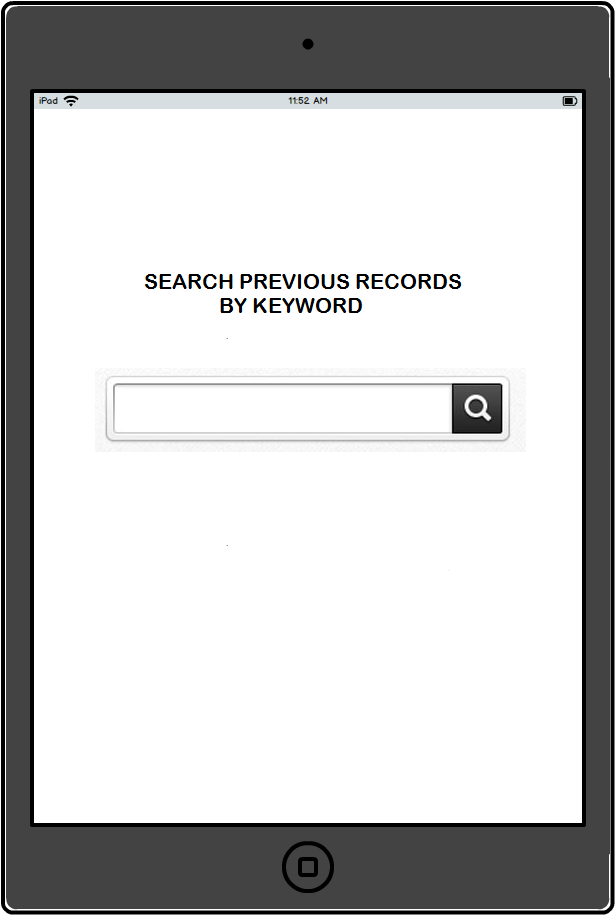
\includegraphics[width=4in,height=6in]{search_mockup.png}
\end{figure}

\newpage
{\selectlanguage{english}\itshape\color{black}
Report look-up selection. 
}
\begin{figure}[H]
\centering
\renewcommand{\figurename}{Report_Lookup}
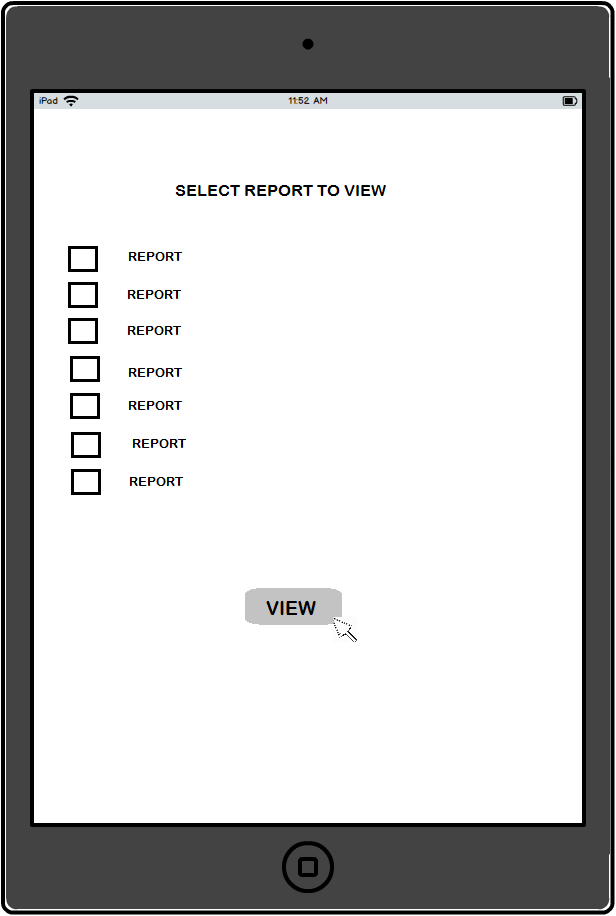
\includegraphics[width=4in,height=6in]{select_report_mockup.png}
\end{figure}

\newpage
{\selectlanguage{english}\itshape\color{black}
Delayed upload screen. 
}
\begin{figure}[H]
\centering
\renewcommand{\figurename}{Delayed_upload}
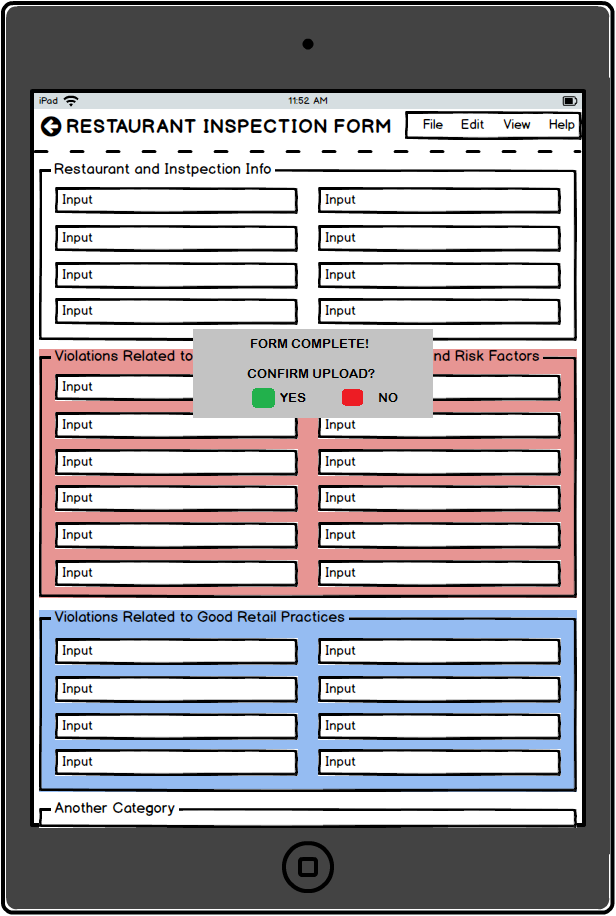
\includegraphics[width=4in,height=6in]{delayed_upload_mockup.png}
\end{figure}

\end{document}
